\documentclass[sigplan]{acmart}

\usepackage{booktabs} % For formal tables


% Copyright
%\setcopyright{none}
%\setcopyright{acmcopyright}
%\setcopyright{acmlicensed}
\setcopyright{rightsretained}
%\setcopyright{usgov}
%\setcopyright{usgovmixed}
%\setcopyright{cagov}
%\setcopyright{cagovmixed}

\usepackage{color}
\usepackage{amssymb,amsmath}
\usepackage{graphicx}
\usepackage{wrapfig}
\usepackage{epsfig}
\usepackage[normalem]{ulem}
\usepackage{url}
\usepackage{hyperref}
\usepackage{color}
\usepackage{array}
\usepackage{subfig}
\usepackage{algorithm,algorithmic}
\usepackage{listings}
%\usepackage[none]{hyphenat} 

\newenvironment{packed_itemize}{
\begin{itemize}
  \setlength{\itemsep}{1pt}
  \setlength{\parskip}{0pt}
  \setlength{\parsep}{0pt}
}{\end{itemize}}

% DOI
\acmDOI{10.1145/3229762.3229767}

% ISBN
\acmISBN{978-1-4503-5923-8}

%Conference
\acmConference[ReQuEST at ASPLOS'18]{1st ACM Reproducible Quality-Efficient Systems Tournament on Co-designing Pareto-efficient Deep Learning}{March 2018}{Williamsburg, VA, USA}
\acmYear{2018}
\copyrightyear{2018}

%\acmPrice{15.00}

%\acmBadgeL[http://ctuning.org/ae/ppopp2016.html]{ae-logo}
%\acmBadgeR[http://ctuning.org/ae/ppopp2016.html]{ae-logo}


\begin{document}

%%%%%%%%%%%%%%%%%%%%%%%%%%%%%%%%%%%%%%%%%%%%%%%%%%%%%%%%%%%%%%%%%%%%%%%%%%%%%%%%%%%%%%%%%%%%%%%%%
\title{Multi-objective autotuning of MobileNets\\ across the full software/hardware stack}

%\titlenote{Produces the permission block, and
%  copyright information}

%\subtitle{Extended Abstract}

%\subtitlenote{The full version of the author's guide is available as
%  \texttt{acmart.pdf} document}

%%%%%%%%%%%%%%%%%%%%%%%%%%%%%%%%%%%%%%%%%%%%%%%%%%%%%%%%%%%%%%%%%%%%%%%%%%%%%%%%%%%%%%%%%%%%%%%%%
\author{Anton Lokhmotov}
%\authornote{}
\affiliation{%
  \institution{dividiti}
}
\email{anton@dividiti.com}

\author{Nikolay Chunosov}
\affiliation{%
  \institution{Xored and dividiti}
}
\email{nikolay.chunosov@xored.com}

\author{Flavio Vella}
%\authornote{}
\affiliation{%
  \institution{dividiti}
}
\email{flavio@dividiti.com}

\author{Grigori Fursin}
\affiliation{%
  \institution{dividiti and cTuning foundation}
}
\email{Grigori.Fursin@cTuning.org}

\renewcommand{\shortauthors}{}
\renewcommand{\shorttitle}{}

%%%%%%%%%%%%%%%%%%%%%%%%%%%%%%%%%%%%%%%%%%%%%%%%%%%%%%%%%%%%%%%%%%%%%%%%%%%%%%%%%%%%%%%%%%%%%%%%%
\begin{abstract}
 We present a customizable Collective Knowledge workflow with
an integrated scoreboard to automate multi-objective benchmarking,
exploration and co-design of diverse machine learning models,
frameworks, libraries and platforms.
%
We demonstrate how it can help to automatically find 
the most efficient stack for image classification 
on a Pareto frontier of accuracy, speed and size 
across MobileNets, TensorFlow, ArmCL OpenCL libraries,
and Arm Mali GPUs.
%
All artifacts, workflows and results from this paper
are shared as open-source, reproducible and reusable components
with a common JSON API for further validation, comparison
and improvement by the community.

These customizable and portable workflows can help enhance 
existing benchmarks such as MLPerf with plug\&play components 
and a live dashboard for a collaborative, reproducible and 
fair comparison of novel techniques, frameworks and platforms.
%
Such approach can help to guide further software and hardware improvements, 
automate Artifact Evaluation at conferences such as SysML, 
and accelerate technology transfer to industry.

\end{abstract}

%%%%%%%%%%%%%%%%%%%%%%%%%%%%%%%%%%%%%%%%%%%%%%%%%%%%%%%%%%%%%%%%%%%%%%%%%%%%%%%%%%%%%%%%%%%%%%%%%
%
% The code below should be generated by the tool at
% http://dl.acm.org/ccs.cfm
% Please copy and paste the code instead of the example below.
%

%\begin{CCSXML}
%\end{CCSXML}

%\ccsdesc[500]{Computer systems organization~Embedded systems}
%\ccsdesc[300]{Computer systems organization~Redundancy}
%\ccsdesc{Computer systems organization~Robotics}
%\ccsdesc[100]{Networks~Network reliability}


%%%%%%%%%%%%%%%%%%%%%%%%%%%%%%%%%%%%%%%%%%%%%%%%%%%%%%%%%%%%%%%%%%%%%%%%%%%%%%%%
\keywords{\small MobileNets, Collective Knowledge, performance, accuracy,
system co-design, reproducible experimentation, customizable workflows,
autotuning, crowdtuning, live scoreboard}

%%%%%%%%%%%%%%%%%%%%%%%%%%%%%%%%%%%%%%%%%%%%%%%%%%%%%%%%%%%%%%%%%%%%%%%%%%%%%%%%
\maketitle

%===============================================================================
\section{Introduction}
\label{sec:intro}
%===============================================================================

MobileNets~\cite{Howard:MobileNets-v1} is a family of efficient convolutional
neural network (CNN) models for mobile and embedded platforms.
%
In theory, using $3 \times 3$ depthwise separable convolutions results in
8--9 times fewer operations than using standard $3 \times 3$ convolutions at a
small loss of accuracy.
%
In practice, the execution time of a model depends on many factors, not
just on the number of operations.

We study performance (execution time and accuracy) trade-offs on two embedded
development platforms (Table~\ref{tab:platforms}).
%
We use TensorFlow~\cite{tensorflow2015-whitepaper} on run MobileNets on the
CPU, and the Arm Compute Library~\cite{arm-compute-library} (ArmCL) to run
MobileNets on the GPU.
%
We use the same set of weights in all experiments (converted into
the ArmCL format for GPU experiments).\footnote{Google released this set of
weights on 14 June 2017. They subsequently released another set on 22 February
2018. Both sets are available as Collective Knowledge components.}

As we have contributed to the ArmCL optimizations for the latest Bifrost GPU
architecture (Mali-G71), we evaluate their effectiveness on the HiKey platform
over several public releases.
%
We also evaluate MobileNets on the Firefly platform with the previous Midgard
GPU architecture (Mali-T860).

To perform experiments across the many combinations of models, libraries, data
sets and hardware, we use a Collective Knowledge workflow for
autotuning~\cite{cm:29db2248aba45e59:c4b24bff57f4ad07}.
%
We make all the workflow components (models, programs, scripts, etc.) publicly
available under the permissive Collective Knowledge license to encourage
further exploration by the community in the spirit of the ACM ReQuEST
tournaments~(Figure~\ref{fig:ck-request-concept}).

%-------------------------------------------------------------------------------
%Figure 1.
%-------------------------------------------------------------------------------
\begin{figure*}[htbp]
% 
  \centering
%
  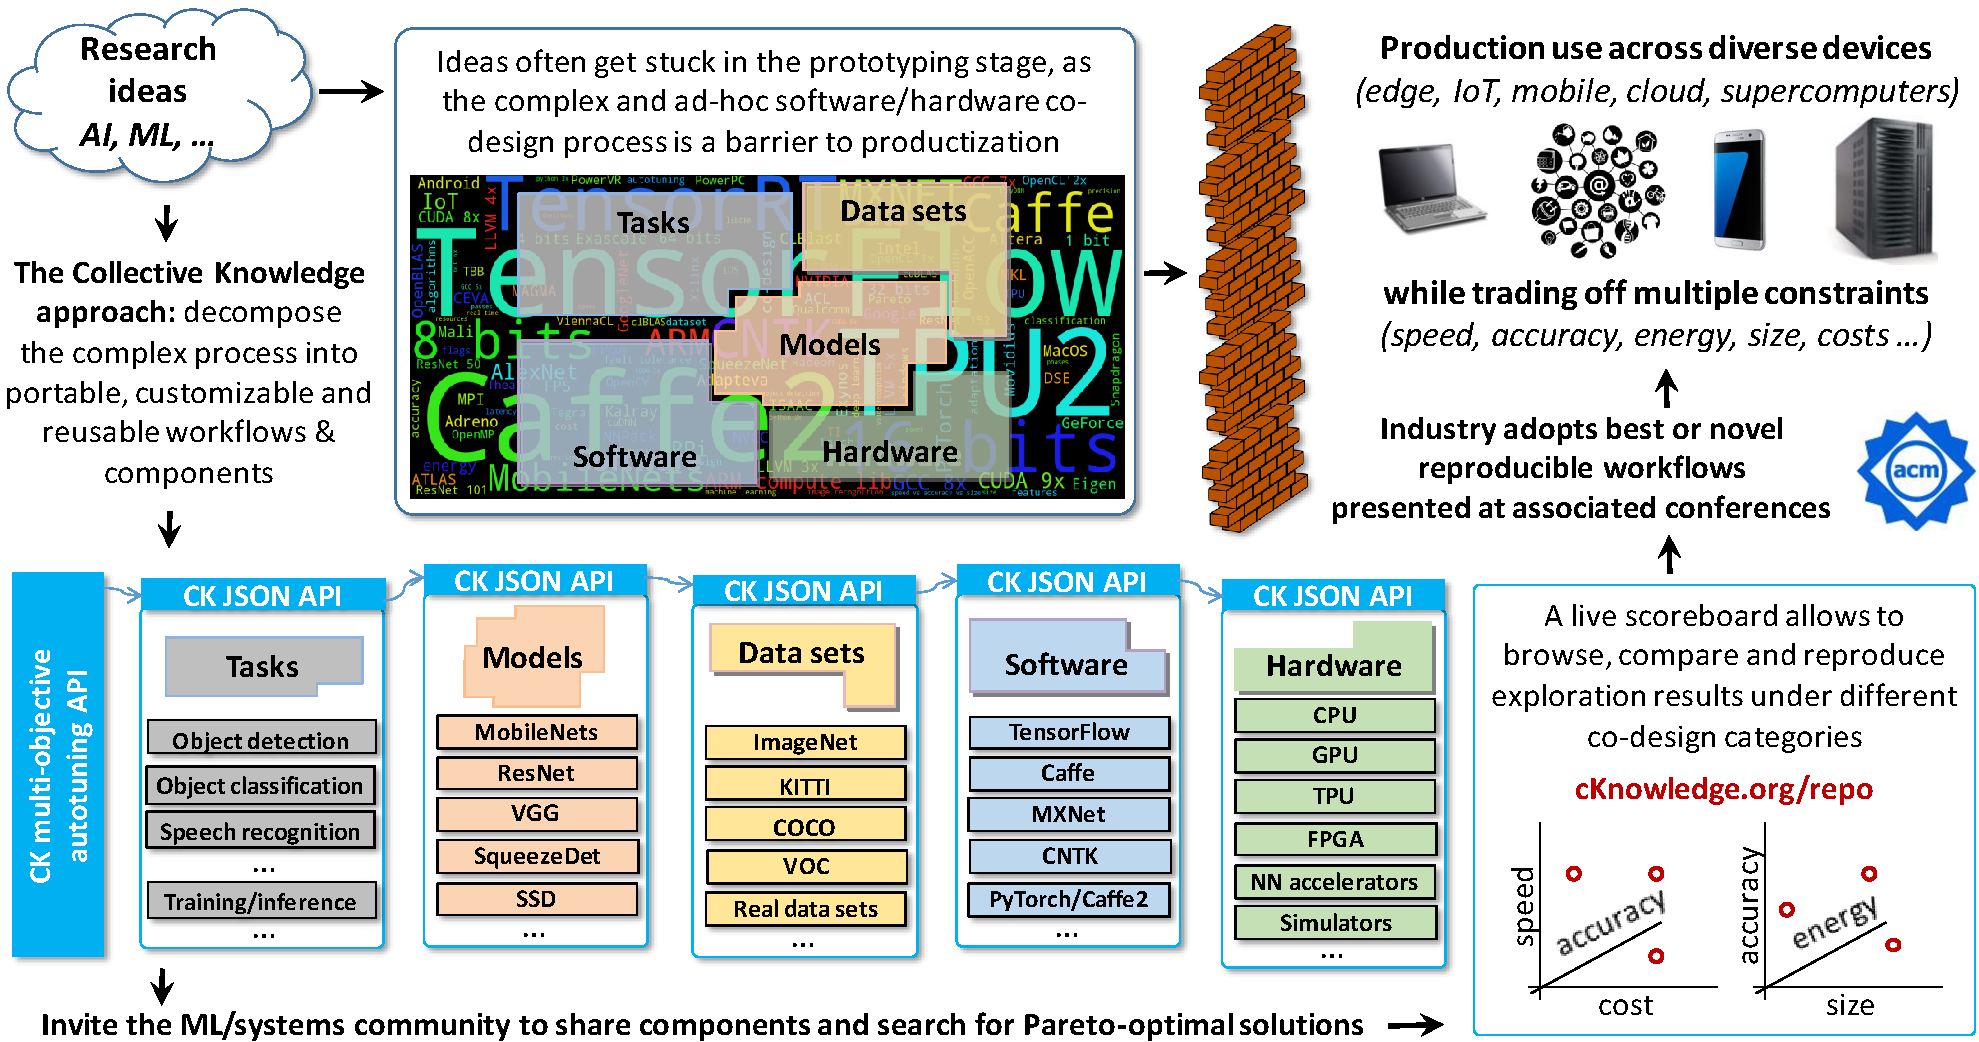
\includegraphics[width=0.9\textwidth]{figures/ck-request-concept-cropped.pdf}
%  
  \caption{The Reproducible Quality-Efficiency Systems Tournaments
(ReQuEST)~\cite{cm:29db2248aba45e59:0c7348dfbadd5b95} invite the
interdisciplinary community to decompose the complex software/hardware
benchmarking, optimization and co-design process into customizable workflows
with reusable components, and collaboratively explore Pareto-efficient
solutions in terms of speed, accuracy, energy, costs and other extensible
metrics across diverse models, data sets, frameworks, libraries and platforms.}
%
  \label{fig:ck-request-concept}
%
\end{figure*}

%-------------------------------------------------------------------------------
% Table 1.
%-------------------------------------------------------------------------------
\begin{table}[htbp]
\centering
  \begin{tabular}{ll}
  \toprule
  \multicolumn{2}{c}{{\bf Linaro HiKey960 (``HiKey'')}}\\
  \midrule
  % https://www.96boards.org/product/hikey960/
  System-on-chip      & HiSilicon Kirin960                      \\
  CPU 0 (``LITTLE'')  & Arm Cortex-A53, 4 cores, $\le$ 1844 MHz \\
  CPU 1 (``big'')     & Arm Cortex-A73, 4 cores, $\le$ 2362 MHz \\
  GPU                 & Arm Mali-G71,   8 cores, $\le$ 1037 MHz \\
  OpenCL              & Specification: 2.0; driver: 6.0         \\
  RAM                 & 3 GiB                                   \\
  \midrule
  % http://en.t-firefly.com/product/rk3399.html
  \multicolumn{2}{c}{{\bf T-Firefly RK3399 (``Firefly'')}}\\
  \midrule
  System-on-chip      & Rockchip RK3399                         \\
  CPU 0 (``LITTLE'')  & Arm Cortex-A53, 4 cores, $\le$ 1416 MHz \\
  CPU 1 (``big'')     & Arm Cortex-A72, 2 cores, $\le$ 1800 MHz \\
  GPU                 & Arm Mali-T860,  4 cores, $\le$  800 MHz \\
  OpenCL              & Specification: 1.2; driver: 13.0        \\
  RAM                 & 4 GiB                                   \\
  \bottomrule
  \end{tabular}
\caption{\label{tab:platforms}Experimental platforms.}
\end{table}

%===============================================================================
\section{Experimental evaluation}
\label{sec:evaluation}
%===============================================================================

\subsection{Parameter space}

The MobileNets family offers two tunable parameters to trade off performance
and accuracy: the input image resolution and the channel
multiplier~\cite{Howard:MobileNets-v1}. 

Additionally, we study the effectiveness of library optimizations over several
ArmCL variants for two convolution methods: {\em direct convolution} computes a
weighted sum of input values ``ab initio''; {\em GEMM-based convolution} uses
an ``image-to-column'' transformation of input values to reduce computation to
a typically highly-optimized generic matrix-matrix multiplication routine
(GEMM).

\subsection{ArmCL Bifrost optimizations}

Our optimizations for the Bifrost GPU architecture first appeared in the v17.12
release of ArmCL.
%
These included writing new OpenCL kernels for most important CNN operators,
restructuring kernels to expose more parallelism and improve locality (e.g.\
kernel fusion), and introducing mechanisms for adaptively selecting the optimal
workgroup size for the given tensor shape.

Unfortunately, our optimizations were mostly disabled in v17.12 due to an issue,
which got fixed in v18.01.
%
As the previous v17.10 release did not support depthwise convolutions, running
MobileNets with v17.12 should give a good approximation of how the models would
perform without our optimizations.

Following the v18.01 release, Arm focused on improving the performance of
GEMM-based convolutions, while we independently developed a new direct $1
\times 1$ convolution kernel. 
%
We integrated this kernel into a fork of v18.03.
%
We refer to this fork as ``dv/dt'' in what follows.

\subsection{Execution time vs.\ top 1 accuracy on HiKey}

Figure~\ref{fig:50000} plots the execution time vs.\ top 1 accuracy over the
full ImageNet validation set (50,000 images) on the HiKey platform with the
following encoding:

% https://github.com/ARM-software/ComputeLibrary/pull/432

\begin{itemize}

  \item The colour of a marker denotes the execution engine: TensorFlow on the CPU or ArmCL on the GPU.

  \item The size of a marker is proportional to the input image resolution: $224$ (the largest), $192$, $160$, $128$ (the smallest).

  \item The shape of a marker denotes both the channel multiplier and the convolution method:
  \begin{itemize}
    \item Direct convolution: $1.00$ - pentagon, $0.75$ - square, $0.50$ - triangle-up, $0.25$ - circle.
    \item GEMM-based convolution: $1.00$ - star, $0.75$ - diamond, $0.50$ - triangle-down, $0.25$ - octagon.\footnote{%
      Roughly speaking, a shape has $N$ corners for the channel multiplier of $(N-1)/4$:
      \begin{itemize}
        \item 5 corners for the channel multiplier of $1.00$ (pentagon or star);
        \item 4 corners for the channel multiplier of $0.75$ (square or diamond);
        \item 3 corners for the channel multiplier of $0.50$ (triangle-up or triangle-down);
        \item ``no corners'' foo the channel multiplier of $0.25$ (circle or octagon).
      \end{itemize}
      }
  \end{itemize}
\end{itemize}

Black crosses mark points lying on a Pareto-optimal frontier. 
%
From any point on the frontier, to increase the accuracy (move up), one must
increase the execution time (move to the right); alternatively, to decrease the
execution time (move to the left), one must decrease the accuracy (move down).

For example, the fastest model (with the input resolution of $128$ and the
channel multipler of $0.25$) takes $10$~ms per input image, but only achieves
the top 1 accuracy of $40.7\%$. 
%
The most accurate model (with the input resolution of $224$ and the channel
multiplier of $1.00$) takes under $50$~ms per image, with the top 1 accuracy of
$70.5\%$.
%
We note that GEMM-based convolution (in v18.03) is faster than the new direct
convolution kernel (``dv/dt'') only for the most accurate model.

\subsection{Top 1 accuracy over 50,000 images}

Given long exploration times for the 16 MobileNets variants over the 50,000
image set, we use the same accuracy for all the ArmCL variants as measured
using v18.03.

As Table~\ref{tab:50000} shows, while this accuracy is similar to the accuracy
measured from a TensorFlow implementation, it is not exactly the same, even
though both implementations use the same set of weights and
preprocessing of input images.
 
Moreover, the measured accuracy is up to $0.8\%$ lower than the accuracy
that the MobileNets authors claimed for the same set of weights.
%
We speculate that this discrepancy is due to a difference in preprocessing of
input images.

%-------------------------------------------------------------------------------
% Figure 2.
%-------------------------------------------------------------------------------
\begin{figure*}[htbp]
  \centering
  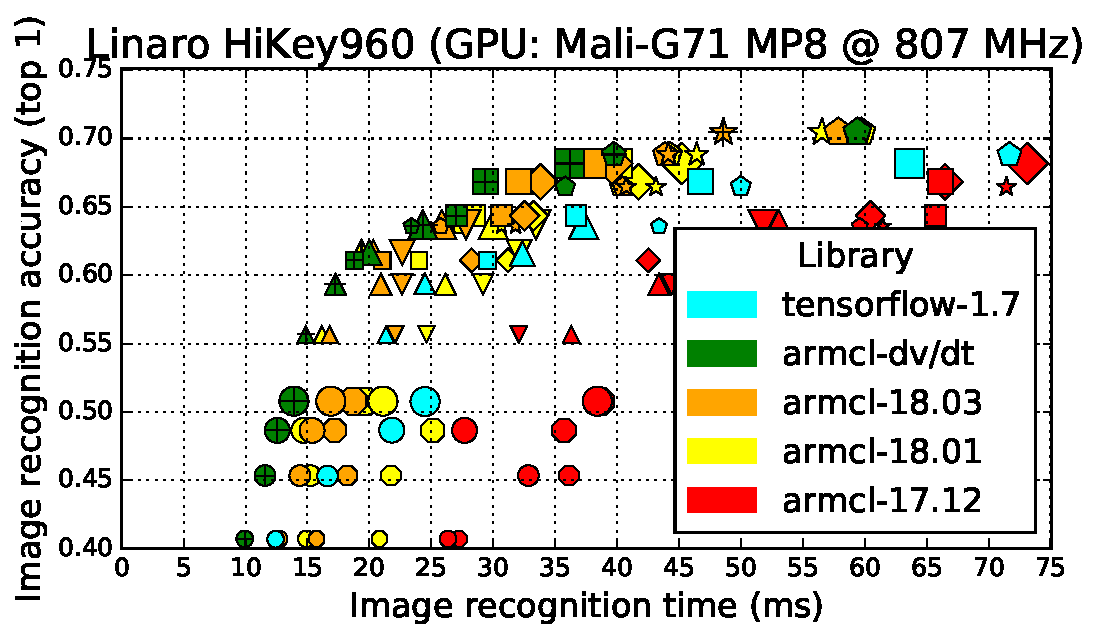
\includegraphics[width=0.95\textwidth]{figures/hikey-960-accuracy_top1_-50000-dv_dt__18_03__18_01__17_12__tf.pdf}
  \caption{Execution time vs.\ top 1 accuracy on 50,000 images (uniform accuracy across all the ArmCL variants).}
  \label{fig:50000}
\end{figure*}


%-------------------------------------------------------------------------------
% Table 2.
%-------------------------------------------------------------------------------
\begin{table}[htbp]
  \centering
  \begin{tabular}{lrrr}
\toprule
{}          & ArmCL     & TensorFlow& TensorFlow \\
MobileNets  & (measured)& (measured)& (claimed)  \\
\midrule
v1-1.00-224 &  0.70464  &  0.70466  &  0.70700   \\
v1-1.00-192 &  0.68830  &  0.68824  &  0.69300   \\
v1-1.00-160 &  0.66458  &  0.66504  &  0.67200   \\
v1-1.00-128 &  0.63586  &  0.63580  &  0.64100   \\
v1-0.75-224 &  0.68172  &  0.68178  &  0.68400   \\
v1-0.75-192 &  0.66840  &  0.66830  &  0.67400   \\
v1-0.75-160 &  0.64350  &  0.64386  &  0.65200   \\
v1-0.75-128 &  0.61096  &  0.61060  &  0.61800   \\
v1-0.50-224 &  0.63690  &  0.63722  &  0.64000   \\
v1-0.50-192 &  0.61674  &  0.61578  &  0.62100   \\
v1-0.50-160 &  0.59354  &  0.59376  &  0.59900   \\
v1-0.50-128 &  0.55674  &  0.55652  &  0.56200   \\
v1-0.25-224 &  0.50794  &  0.50766  &  0.50600   \\
v1-0.25-192 &  0.48658  &  0.48676  &  0.49000   \\
v1-0.25-160 &  0.45354  &  0.45322  &  0.46000   \\
v1-0.25-128 &  0.40724  &  0.40694  &  0.41300   \\
\bottomrule
\end{tabular}

  \caption{Top 1 accuracy on 50,000 images. The data in the last column was taken from an older version of the MobileNets page on GitHub: \url{https://github.com/tensorflow/models/blob/1630da3434974e9ad5a0b6d887ac716a97ce03d3/research/slim/nets/mobilenet_v1.md} (which presumably corresponds to the set of weights released on 14 June 2017).}
  \label{tab:50000}
\end{table}

%-------------------------------------------------------------------------------
\subsection{Top 1 accuracy over 500 images}
%-------------------------------------------------------------------------------

Consider the top row of Table~\ref{tab:50000}.
%
A discrepancy of $0.0002$ (equivalent to 1 image out of 50,000) measured between ArmCL and TensorFlow might not sound much.
%
A closer investigation over the first 500 images in this data set, however,
revealed 3 cases in which the ArmCL implementation classified images
differently from the TensorFlow one.
%
In all these cases, TensorFlow predicted the top class correctly, while ArmCL predicted
the correct class as the second most likely.
%
From the overall discrepancy of $0.0002$, it follows that there existed cases
where ArmCL predicted the top class correctly, while TensorFlow did not.
%
Such cases could be of great interest to numerical analysts.
%

\begin{table*}[htb]
  \centering
  \begin{tabular}{l|l}
  \toprule
  {\bf ArmCL predictions} & {\bf TensorFlow predictions} \\
  \midrule
  \midrule
  \multicolumn{2}{l}{ILSVRC2012\_val\_00000060.JPEG - (588) n03482405 hamper} \\
  \midrule
  0.45 - (492) n03014705 chest                              &  0.47 - (588) n03482405 hamper                              \\
  0.45 - (588) n03482405 hamper                             &  0.43 - (492) n03014705 chest                               \\ 
  0.02 - (626) n03666591 lighter, light, igniter, ignitor   &  0.02 - (626) n03666591 lighter, light, igniter, ignitor    \\
%  0.01 - (526) n03179701 desk                               &  0.01 - (526) n03179701 desk                                \\
%  0.01 - (681) n03832673 notebook, notebook computer        &  0.01 - (681) n03832673 notebook, notebook computer         \\
  \midrule
  \multicolumn{2}{l}{ILSVRC2012\_val\_00000302.JPEG - (469) n02939185 caldron, cauldron} \\
  \midrule
  0.48 - (926) n07590611 hot pot, hotpot                    &  0.47 - (469) n02939185 caldron, cauldron                   \\
  0.47 - (469) n02939185 caldron, cauldron                  &  0.47 - (926) n07590611 hot pot, hotpot                     \\
  0.02 - (925) n07584110 consomme                           &  0.02 - (925) n07584110 consomme                            \\
%  0.01 - (996) n13052670 hen-of-the-woods                   &  0.01 - (996) n13052670 hen-of-the-woods                    \\
%  0.01 - (809) n04263257 soup bowl                          &  0.01 - (809) n04263257 soup bowl                           \\
  \midrule
  \multicolumn{2}{l}{ILSVRC2012\_val\_00000313.JPEG - (979) n09468604 valley, vale} \\
  \midrule
  0.18 - (984) n11879895 rapeseed                           &  0.17 - (979) n09468604 valley, vale                        \\
  0.17 - (979) n09468604 valley, vale                       &  0.17 - (984) n11879895 rapeseed                            \\
  0.11 - (978) n09428293 seashore, coast, seacoast          &  0.12 - (978) n09428293 seashore, coast, seacoast           \\
%  0.09 - (525) n03160309 dam, dike, dyke                    &  0.09 - (525) n03160309 dam, dike, dyke                     \\
%  0.07 - (483) n02980441 castle                             &  0.07 - (975) n09332890 lakeside, lakeshore                 \\
  \bottomrule
  \end{tabular}

  \caption{Image classification differences between ArmCL~v18.03 and
TensorFlow~v1.7 over the first 500 images in the ImageNet validation set. For
each image, the correct label is shown against its file name; below, the top 3
predictions according to ArmCL (left column) and TensorFlow (right column) are
shown together with their probabilities.}

  \label{tab:500}
\end{table*}

Having observed the differences between ArmCL and TensorFlow, we measured the
accuracy over the same 500 images for all the ArmCL variants on HiKey
(Figure~\ref{fig:500:hikey}) and Firefly (Figure~\ref{fig:500:firefly}).
%
On both platforms, the results were identical to v18.03, except for v17.12.
%
With v17.12, only the models with the input resolution of $128$ produced the same
results. For the other input resolutions, the differences ranged from $5.8\%$
to $58.6\%$ on HiKey and from $7.2\%$ to $59.4\%$ on Firefly, with differences
also between the GEMM-based and direct convolution approaches.
%
This clearly indicated a platform-independent issue in v17.12.
%
Had it not got fixed in v18.01, this information could have been useful for
debugging.
%

\begin{figure*}[tp]
  \centering
   \subfloat[HiKey.\label{fig:500:hikey}]{%
    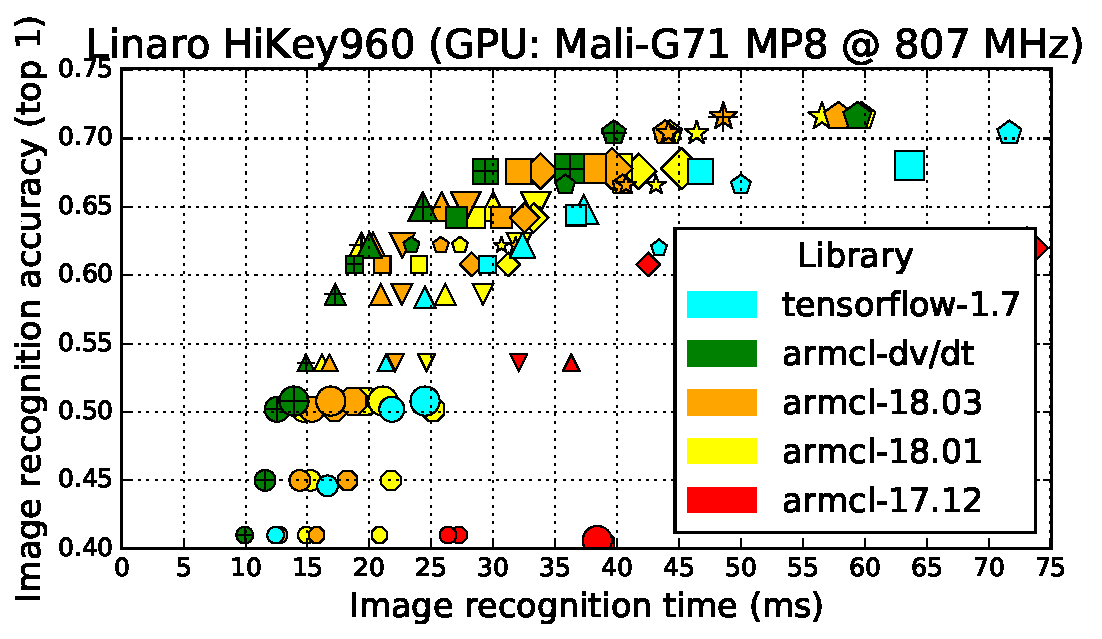
\includegraphics[width=0.95\textwidth]{figures/hikey-960-accuracy_top1-500-dv_dt__18_03__18_01__17_12__tf.pdf}
  }
  \hfill
  \subfloat[Firefly.\label{fig:500:firefly}]{%
    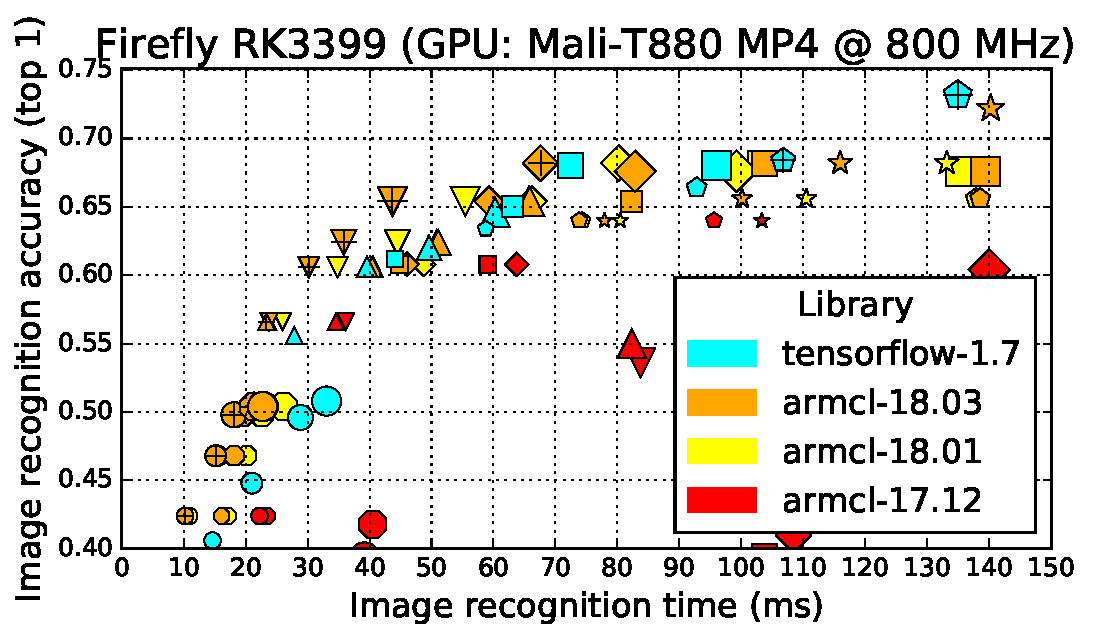
\includegraphics[width=0.95\textwidth]{figures/firefly-accuracy_top1-500-18_03__18_01__17_12__tf.pdf}
  }
  \caption{Execution time vs.\ top 1 accuracy on 500 images.\label{fig:500}}
\end{figure*}

Finally, we observed differences between the platforms. 
%
For example, the model with the input resolution of $128$ and the channel
multiplier of $0.50$ scored $53.6\%$ with ArmCL and TensorFlow on HiKey but
$56.6\%$ with ArmCL and $55.6\%$ with TensorFlow on Firefly.

%-------------------------------------------------------------------------------
\subsection{Execution time on HiKey and Firefly}
%-------------------------------------------------------------------------------

Figure~\ref{fig:500} can also be studied to compare the experimental platforms.
%
On purpose, the X axis extends to 75~ms in Figure~\ref{fig:500:hikey} and to
150~ms in Figure~\ref{fig:500:firefly}, since HiKey has twice as many GPU cores
and ``big'' CPU cores as Firefly (see Table~\ref{tab:platforms}).
%

On the one hand, HiKey tends to be less efficient per GPU core than Firefly for
the models with the channel multipliers of $0.25$ and $0.50$. 
%
For example, the least accurate model takes 10~ms on both platforms.
%
This is likely due to the limited parallelism of the workload.

On the other hand, HiKey is up to $50\%$ more efficient per GPU core (3 times
faster) than Firefly for the models with the channel multiplier of $1.00$.
%
This is likely due to the innate architectural differences between the newer
Bifrost and older Midgard GPU architectures.

%===============================================================================
\section{Conclusion and future work}
%===============================================================================

We have retargeted a customizable and portable Collective Knowledge autotuning
workflow from~\cite{cm:29db2248aba45e59:c4b24bff57f4ad07} to study the performance
and accuracy trade-offs of the MobileNets family across many combinations of
parameters, libraries, data sets and platforms. 
%
For example, by sacrificing $7\%$ of the accuracy, the execution time of the
most accurate model can be reduced by 2 times on HiKey and by 3 times on
Firefly; even more dramatically, by sacrificing $30\%$ of the accuracy, the
execution time can be reduced by 5 times on HiKey and by 14 times on Firefly.

Our study highlights the challenge of maintaining the accuracy when deploying
CNN models across diverse platforms.
%
We have observed up to $3\%$ differences when using the same set of 32-bit
floating point weights across libraries and platforms.
%
This challenge will only intensify when considering aggressive optimization
techniques such as weights pruning and quantization.

The presented Collective Knowledge workflow can be extended to support:
\begin{itemize}

  \item further autotuning choices such as the batch size, processor frequency, numerical precision, etc.;

  \item further autotuning objectives such as power consumption, memory usage and hardware cost;

  \item other models for resource-constrained platforms such as MobileNets-v2~\cite{Sandler:MobileNets-v2}, SqueezeNet~\cite{Iandola:SqueezeNet}, etc.;

  \item emerging hardware platforms with neural network acceleration such as Linaro's HiKey970, Rock960 and Ultra96 development boards;\footnote{\url{https://www.96boards.ai/}}

  \item Google's Android Neural Networks API\footnote{\url{https://developer.android.com/ndk/guides/neuralnetworks}} and TensorFlow Lite;\footnote{\url{https://www.tensorflow.org/mobile/tflite}}

  \item vendor-specific frameworks such as Arm's Neural Network SDK,\footnote{\url{https://developer.arm.com/products/processors/machine-learning/arm-nn}} Qualcomm's Snapdragon Neural Processing Engine,\footnote{\url{https://developer.qualcomm.com/software/qualcomm-neural-processing-sdk}} Huawei's HiAi Computing Platform,\footnote{\url{http://developer.huawei.com/consumer/en/service/HiAI.html}} etc.

\end{itemize}

We humbly hope that our artifact can serve as a blueprint for future ReQuEST
submissions, as well as considered for inclusion into other community-driven
initiatives such as MLPerf~\cite{mlperf}.


%===============================================================================
% Acknowledgements.
%===============================================================================
\begin{acks} 

We thank Anthony Barbier, Georgios Pinitas, Gian Marco Iodice, Peter Horsman
and Jim Chaney from Arm, and Daniil Efremov and Dmitry Savenko from Xored for
collaboration on optimizing deep learning operators for the Arm Bifrost GPU
architecture.

\end{acks}
%===============================================================================


%===============================================================================
% Bibliography.
%===============================================================================
\bibliographystyle{ACM-Reference-Format}
\bibliography{paper}
%===============================================================================


%===============================================================================
% Appendix
%===============================================================================
\appendix
\clearpage
\newpage
\pagebreak
%CK_APPENDIX={A}%
\onecolumn

\section{Artifact Appendix}
\label{artifact_appendix}

Submission and reviewing methodology: \\
{\em http://cTuning.org/ae/submission-20171101.html}

%%%%%%%%%%%%%%%%%%%%%%%%%%%%%%%%%%%%%%%%%%%%%%%%%%%%%%%%%%%%%%%%%%%%%
\subsection{Abstract}

This Artifact Appendix describes experimental workflow,
artifacts and results from this paper evaluated 
during the 1st reproducible ReQuEST tournament at the ACM ASPLOS'18:

\begin{packed_itemize}
  \item {\bf Latest CK workflow:} \url{https://github.com/dividiti/ck-request-asplos18-mobilenets-armcl-opencl}
  \item {\bf CK results:} \url{https://github.com/ctuning/ck-request-asplos18-results-mobilenets-armcl-opencl}
  \item {\bf Artifact DOI:} \url{https://doi.org/10.1145/3229773}
  \item {\bf ReQuEST submission and reviewing guidelines:} \url{http://cknowledge.org/request-cfp-asplos2018.html} (\cite{request-asplos18})
  \item {\bf ReQuEST goals:} \cite{cm:29db2248aba45e59:0c7348dfbadd5b95}
  \item {\bf ReQuEST workflows:} \url{https://github.com/ctuning/ck-request-asplos18-results}
  \item {\bf ReQuEST scoreboard:} \url{http://cKnowledge.org/request-results}
\end{packed_itemize}

%%%%%%%%%%%%%%%%%%%%%%%%%%%%%%%%%%%%%%%%%%%%%%%%%%%%%%%%%%%%%%%%%%%%%
\subsection{Artifact check-list}

Details: \url{http://cTuning.org/ae/submission_extra.html}

\begin{packed_itemize}
  \item {\bf Algorithm:} image classification
  \item {\bf Program:} MobileNets using Arm Compute Library v17.12+ and TensorFlow 1.7.0+
  \item {\bf Compilation:} GCC v6+ (recommended v7+); Python 2.7+ or 3.4+
  \item {\bf Transformations:}
  \item {\bf Binary:} compiled from source on a target platform
  \item {\bf Data set:} ImageNet 2012 validation (50,000 images)
  \item {\bf Run-time environment:} Linux; OpenCL v1.2+
  \item {\bf Hardware:} Linaro HiKey960, Firefly RK3399 development boards (or similar)
  \item {\bf Run-time state:} CPU and GPU frequencies set to the maximum
  \item {\bf Execution:} 
  \item {\bf Metrics:} total execution time; top1/top5 accuracy over some (all) images from the data set
  \item {\bf Output:} classification result; execution time (throughput/latency) versus accuracy
  \item {\bf Experiments:} automated via CK command line
  \item {\bf How much disk space required (approximately)?} 4..20GB depending on library installations
  \item {\bf How much time is needed to prepare workflow (approximately)?} from 30 minutes to 1 day (if natively building TF)
  \item {\bf How much time is needed to complete experiments (approximately)?} from 30 minutes to 1 week (if validating accuracy on complete data set)
  \item {\bf Publicly available?:} Yes
  \item {\bf Code license(s)?:} BSD 3-clause
  \item {\bf CK workflow framework used?} Yes
  \item {\bf CK workflow URL:} \url{https://github.com/dividiti/ck-request-asplos18-mobilenets-armcl-opencl}
  \item {\bf CK results URL:} \url{https://github.com/ctuning/ck-request-asplos18-results-mobilenets-armcl-opencl}
\end{packed_itemize}

%-------------------------------------------------------------------------------
\subsection{Description}

\subsubsection{How to obtain}

\textbf{NB:} Execute commands prefixed with `\#` sign under `root` or using `sudo`.

First, install CK workflow framework:

\begin{verbatim}
# apt install python python-pip
# pip install ck
\end{verbatim}

Alternatively, you can install the latest CK version in a user space from GitHub:
\begin{verbatim}
$ git clone http://github.com/ctuning/ck
$ export PATH=$PWD/ck/bin:$PATH
$ export PYTHONPATH=$PWD/ck:$PYTHONPATH
\end{verbatim}

\noindent Then, install CK repositories:
\begin{verbatim}
$ ck pull repo --url=https://github.com/dividiti/ck-request-asplos18-mobilenets-armcl-opencl
\end{verbatim}

\subsubsection{Install this CK workflow from the ACM Digital Library snapshot}

It is possible to install and test the snapshot of this workflow 
from the ACM Digital Library without interfering with your current CK installation.
Download related file "request-asplos18-artifact-?-ck-workflow.zip"
to a temporary directory, unzip it and then execute the following commands:

\begin{verbatim}
$ . ./prepare_virtual_ck.sh
$ . ./start_virtual_ck.sh
\end{verbatim}

All CK repositories will be installed in your current directory.
You can now proceed with further evaluation as described below.

%-------------------------------------------------------------------------------
\subsubsection{Hardware dependencies}

The new direct convolution kernel optimized for the Arm Mali Bifrost GPU
architecture can be evaluated on a Mali-G71 GPU (e.g.\ found in the HiSilicon
Kirin 960 chip) or Mali-G72 GPU (e.g.\ found in the HiSilicon Kirin 970 chip).
%
The workflow, however, can also be tested on any Arm Mali GPU with the Arm Mali
Midgard GPU architecture (e.g.\ Mali-T880 found in the Rockchip RK3399 chip).

%-------------------------------------------------------------------------------
\subsubsection{Software dependencies}

Software dependencies for CK workflows are automatically installed and rebuilt 
via shared CK packages: \url{https://github.com/ctuning/ck/wiki/Shared-packages}.

However, they may still require some native packages:

\paragraph{ArmCL}

\begin{verbatim}
# apt install libblas-dev liblapack-dev libatlas-base-dev
# apt install python-numpy python-scipy
# pip install pillow
\end{verbatim}

\paragraph{TensorFlow}

\begin{verbatim}
# apt install liblapack-dev libatlas-dev
# pip install enum34 mock pillow wheel absl-py scipy
$ ck install ck-env:package:jdk-8u131-universal
$ ck install ck-env:package:tool-bazel-0.11.1-linux
\end{verbatim}

%-------------------------------------------------------------------------------
\subsubsection{Data sets}

\begin{verbatim}
$ ck install package:imagenet-2012-val-min-resized
$ ck install package:imagenet-2012-aux
\end{verbatim}

\paragraph{ArmCL}

\begin{verbatim}
$ ck install package --tags=mobilenet-v1-all,npy
\end{verbatim}

\paragraph{TensorFlow}

\begin{verbatim}
$ ck install package \
  --tags=mobilenet-v1-all,tensorflowmodel,2017_06_14 
\end{verbatim}


%%%%%%%%%%%%%%%%%%%%%%%%%%%%%%%%%%%%%%%%%%%%%%%%%%%%%%%%%%%%%%%%%%%%%
\subsection{Installation}

\paragraph{ArmCL}

\begin{verbatim}
$ ck install package:lib-armcl-opencl-request
$ ck install package:lib-armcl-opencl-18.03 \
  --env.USE_GRAPH=ON --env.USE_NEON=ON
\end{verbatim}

\paragraph{TensorFlow}

\begin{verbatim}
$ ck install package:lib-tensorflow-1.7.0-src-cpu \
  --env.CK_HOST_CPU_NUMBER_OF_PROCESSORS=1
\end{verbatim}


%%%%%%%%%%%%%%%%%%%%%%%%%%%%%%%%%%%%%%%%%%%%%%%%%%%%%%%%%%%%%%%%%%%%%
\subsection{Experiment workflow}

\paragraph{ArmCL}

\begin{verbatim}
$ cd `ck find script:mobilenets-armcl-opencl`
$ python benchmark.py [--repetitions=10]
$ python benchmark.py --accuracy
\end{verbatim}

\paragraph{TensorFlow}

\begin{verbatim}
$ cd `ck find script:mobilenets-tensorflow`
$ python benchmark.py [--repetitions=10]
$ python benchmark.py --accuracy
\end{verbatim}


%%%%%%%%%%%%%%%%%%%%%%%%%%%%%%%%%%%%%%%%%%%%%%%%%%%%%%%%%%%%%%%%%%%%%
\subsection{Evaluation and expected result}

\begin{verbatim}
$ ls `ck find jnotebook:mobilenets-armcl-opencl`
analysis.ipynb
\end{verbatim}

%%%%%%%%%%%%%%%%%%%%%%%%%%%%%%%%%%%%%%%%%%%%%%%%%%%%%%%%%%%%%%%%%%%%%
\subsection{Notes}

We suggest to check the ReadME from the live CK workflow 
for the latest installation and usage instructions: 

\url{https://github.com/dividiti/ck-request-asplos18-mobilenets-armcl-opencl} .

%===============================================================================

\end{document}
